\documentclass[12pt]{article}

\usepackage{graphicx}

\title{An approach to breast tumor classification using an active learning method}


\author{Shaan Varia \\ Carnegie Mellon University \and Akul Penugonda \\ Carnegie Mellon University}

\begin{document}

\maketitle

\section{Introduction}

Currently, the scenario in an oncologist's room is thus: a patient enters with a potential tumor, which is diagnosed by a doctor as either possibly malignant or non-malignant. If possibly malignant, a biopsy is performed to verify. A biopsy can cost anywhere from \$150 to \$10000. It is a painfully invasive procedure which should be avoided if possible, for both cost and comfort. A machine learning approach could result in a lot of saved money and pain. In this paper, we discuss an application of DHM to a mammographic mass dataset, using only features which may be acquired by non-invasive methods.  Our results show that DHM 's learning approaches the accuracy of a supervised learner, indicating potential benefits to using this in the real world.

\section{Background}



\subsection{Related Work}

\section{Methods}

\subsection{Data Source}

We will get our data from the UCI machine learning repository. The below data set has 961 entries, where each entry contains the following features and labellings: 

6 Attributes in total (1 goal field, 1 non-predictive, 4 predictive attributes) 

1. BI-RADS assessment: 1 to 5 (ordinal, non-predictive!) 
2. Age: patient's age in years (integer) 
3. Shape: mass shape: round=1 oval=2 lobular=3 irregular=4 (nominal) 
4. Margin: mass margin: circumscribed=1 microlobulated=2 obscured=3 ill-defined=4 spiculated=5 (nominal) 
5. Density: mass density high=1 iso=2 low=3 fat-containing=4 (ordinal) 
6. Severity: benign=0 or malignant=1 (binominal, goal field!) 

Taken from https://archive.ics.uci.edu/ml/datasets/Mammographic+Mass 

We will not use BI-RADS as it is too predictive of a feature, we will instead just use Age, Shape, Margin and Density to predict Severity.

\subsection{Features}

We will write an active learner which looks at four features obtained from a mammogram of the breast. These four features are age of patient, shape of breast, margin of breast, and density of breast. We will use these to predict severity, i.e. whether the mass in the patients breast is benign or malignant. Before discussing the learner, we will go over the role that each of these features play in relation to the mass observed being malignant or benign.

\begin{itemize}

\item Density

Density of mammographic mass does not refer to the traditional definition of density (mass/volume), rather it refers to the amount of fat and tissue in the breast. A dense breast is one that has more tissue than fat. Studies have shown that women with high breast density are 4-5 times more likely to develop breast cancer compared to women with low breast density [1]. 

Density is an ordinal field, that is, the higher the density the higher the chance of the mass being malignant.

\item Margin

Margin refers to what the outer part of the mass looks like. Margin of the mammographic mass is a nominal field, and as such we will go into the distinctions between the classes. 

\begin{itemize}

\item Circumscribed

The mass is surrounded by tissue and is not as likely to be malignant, most circumscribed margins are likely to be benign [2,3].

\item Microlobulated

Microlobulated breast margins refer to many small lobulations on the surface of a breast nodule. If more of these microlobulations pop up on the mass then there is a higher chance of the mass being malignant [4], and as such microlobulated masses are treated with more care, and are not simply passed off as benign.

\item Obscured

Obscured breast margins are suspicious due to the fact that they cannot be discerned.
Ill-defined/Irregular
An ill defined margin is one that cannot be distinguished from the fatty tissue surrounding it. This may mean that the mass is invading the tissue, which would be an indicator of malignancy.

\end{itemize}

\item Shape

Shape is similarly a nominal field, and simply refers to the visual shape of the mass as observed on the mammogram.
Round, Oval, Lobular
All of these shapes are not highly indicative of malignancy. Lobular masses refer to those who have small undulations on the mammogram.
Irregular
Irregular masses are indicative of malignancy by virtue of the fact that they are not the regular shapes of common benign masses such as fibroadenomas or cysts.

\end{itemize}

\subsection{Active Learning}



\section{Results}

\begin{figure}
	\centering
	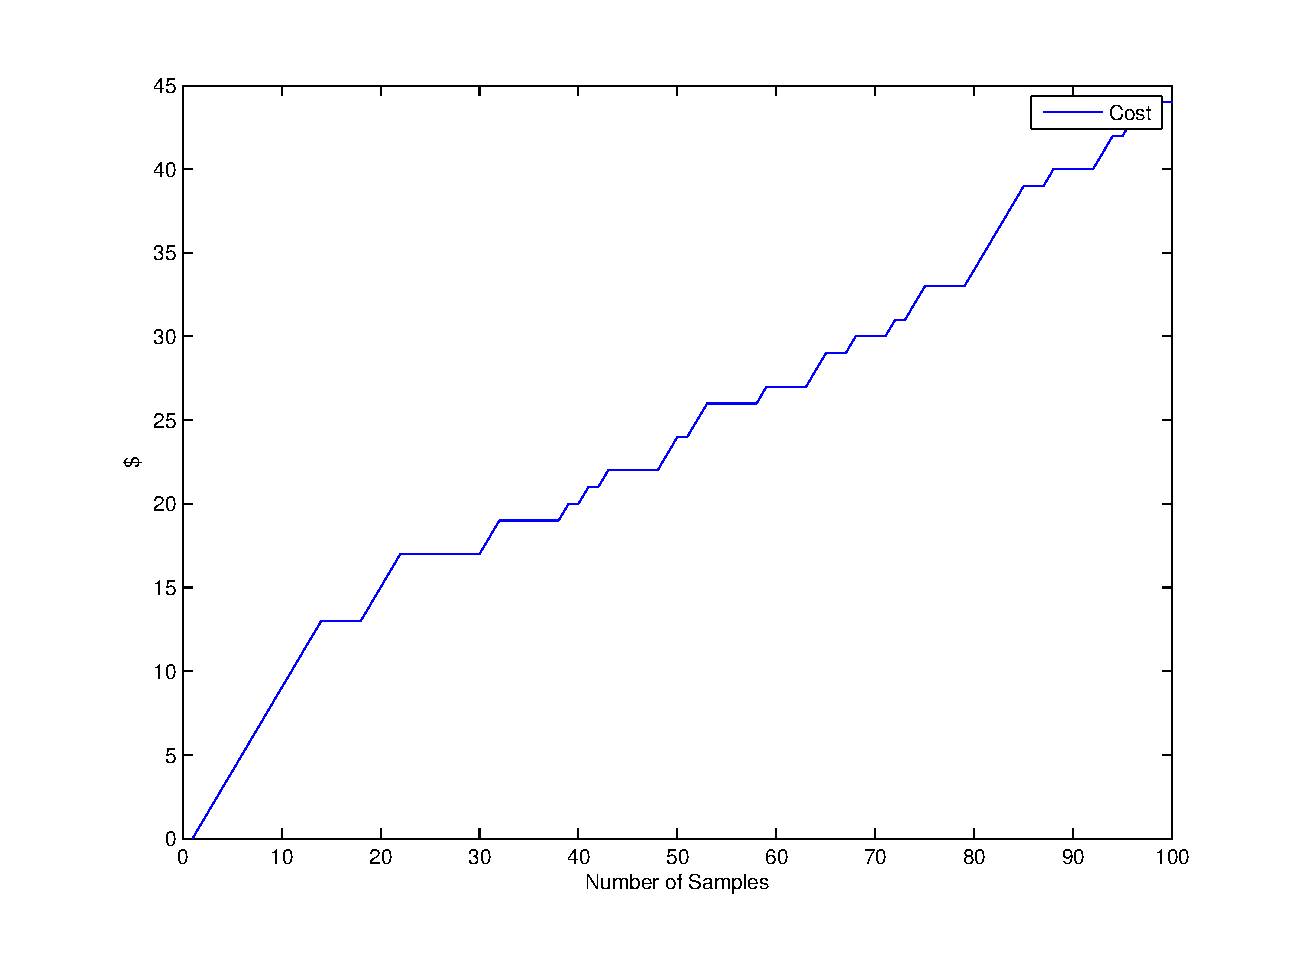
\includegraphics[width=300px]{costcurve}
	\caption{Cost Curve}
	\label{fig:costcurve}
\end{figure}

\begin{figure}
	\centering
	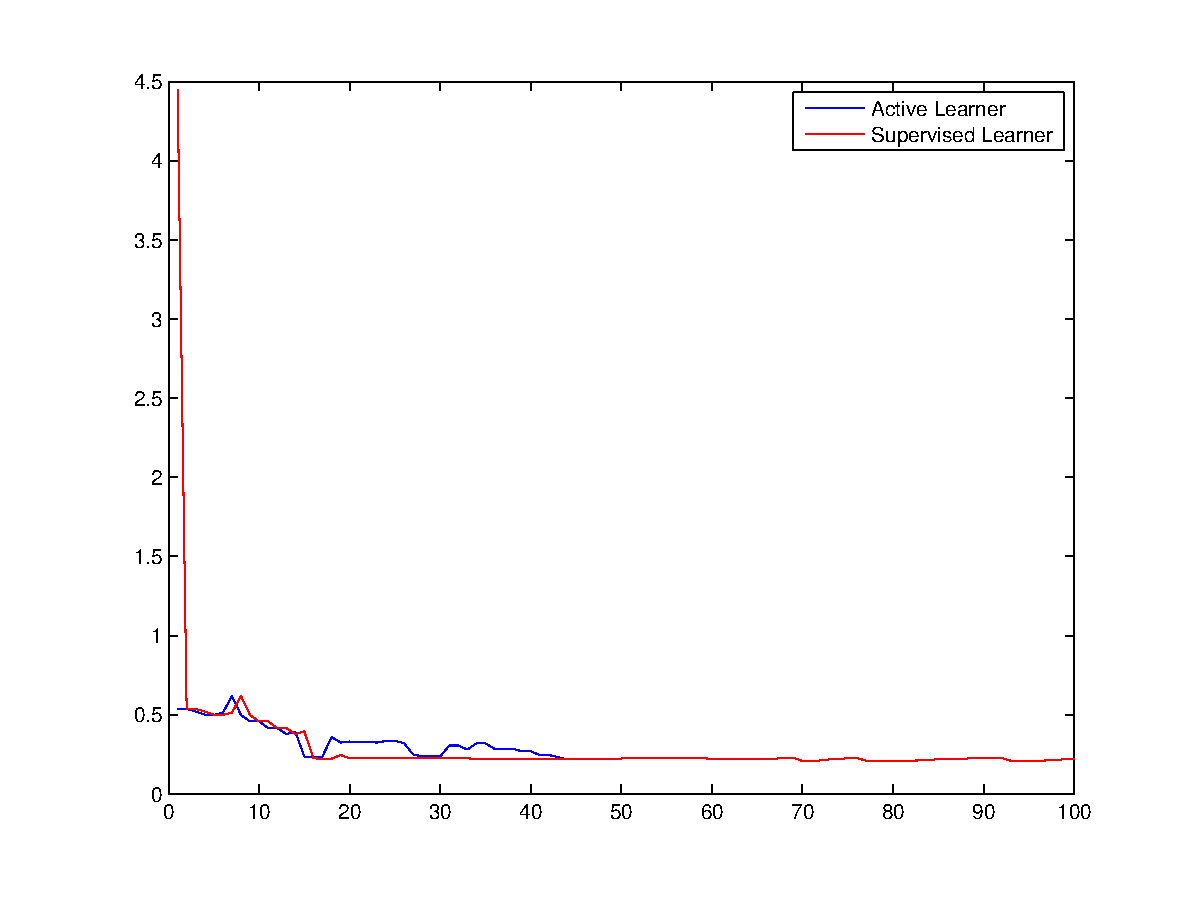
\includegraphics[width=300px]{generr}
	\caption{Generalized Error}
	\label{fig:generr}
\end{figure}

\begin{figure}
	\centering
	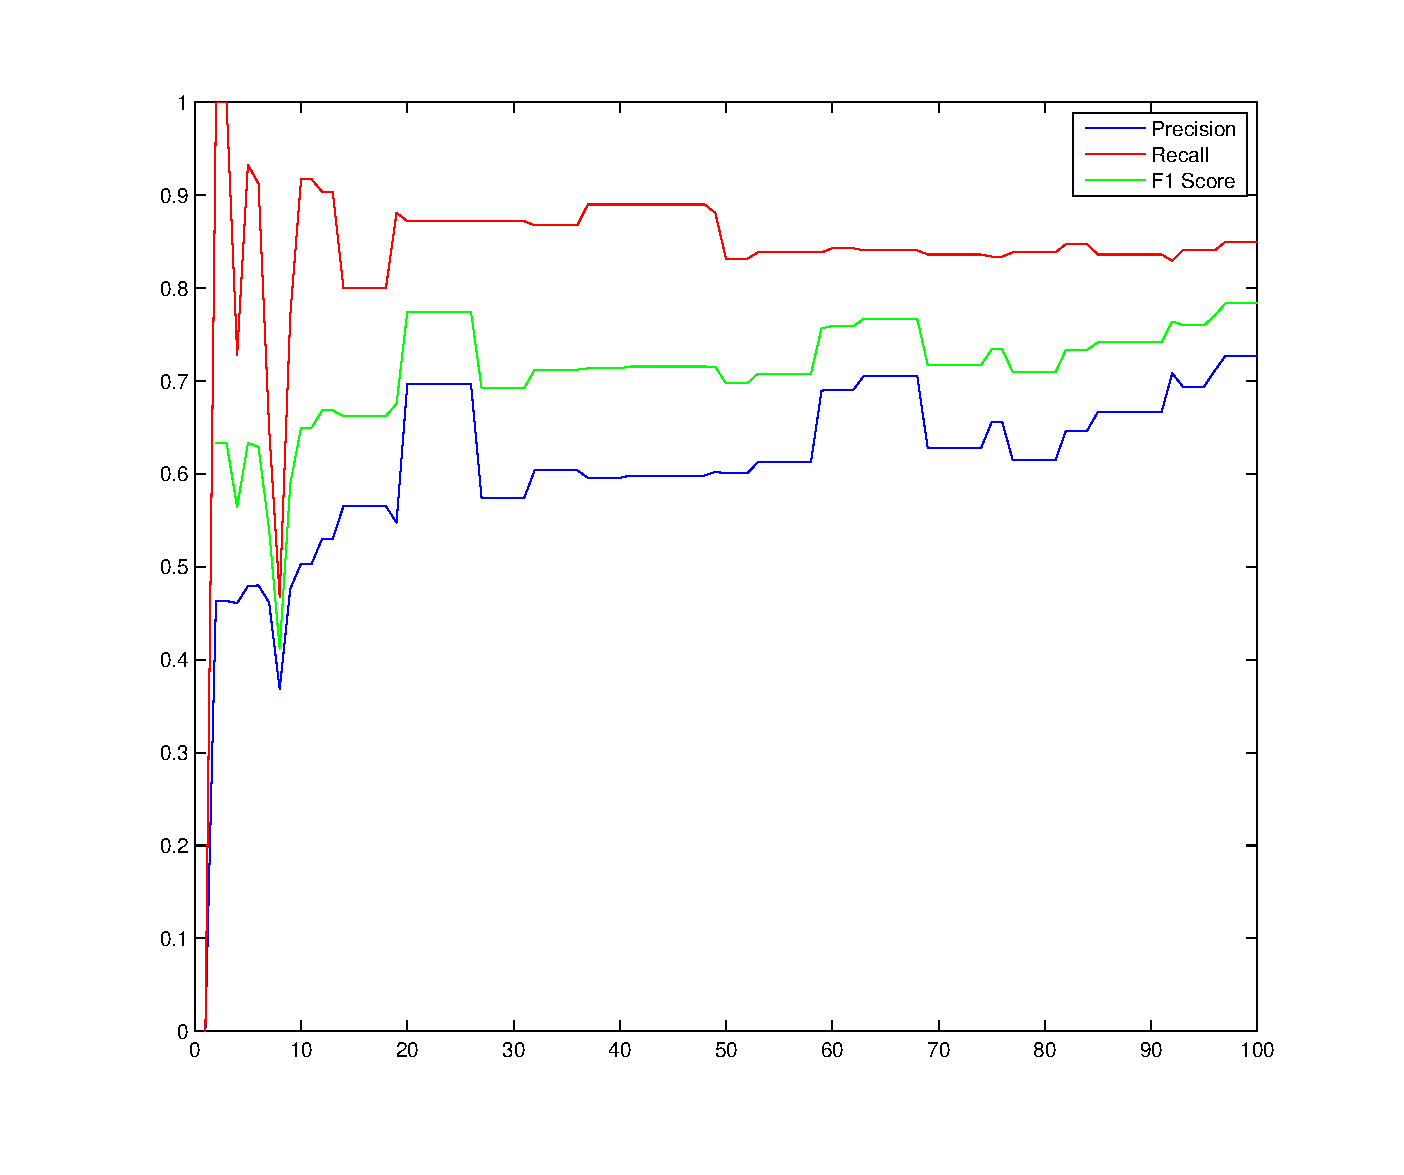
\includegraphics[width=300px]{precisionrecall}
	\caption{Generalized Error}
	\label{fig:precisionrecall}
\end{figure}

\section{Discussion}

\section{Results}

\subsection{Future Work}

\end{document}